\subsection{Iteration 1}

\subsubsection{Define Precisely}

\paragraph*{Classification of Organizational Structures}

To precisely define our problem, we first need to define a taxonomy of organizational structures in order give a common way of describing these structures. To this end, we agree with Rockart, Earl and Ross~\cite{Rockart1996} who describe a continuum of IT governance styles ranging from centralized to decentralized, with federalism in the middle. Many organizations today tend to combine both centralization and decentralization in order to obtain the advantages of both styles: global integration and efficiency due to centralized management in some key areas and agility and high quality of local customer services due to decentralized decision making in others. 

For the purpose of this thesis work, three types of organizational structure in IT are considered along a centralization continuum: \textit{Centralized IT}, where all IT related decisions are made in a centralized manner by the top-level executives, \textit{Decentralized IT}, where each organizational subunit manages its IT in completely autonomous and independent manner,  and \textit{Federal IT} that can be seen as a combination of central IT management and IT management in the subunits. Here a primary task  would be to maintain standards for the entire enterprise while supporting flexibility on the subunit level. The business units would still have ownership of many of their own systems, allowing them to implement them as they deem best. 

Figure \ref{fig:taxonomy} maps the organizational forms presented in Section \ref{sec:organizations} to the continuum, ranging them from highly centralized (e.g. bureaucratic) to decentralized (e.g. virtual organizations).

\begin{figure}
\centering
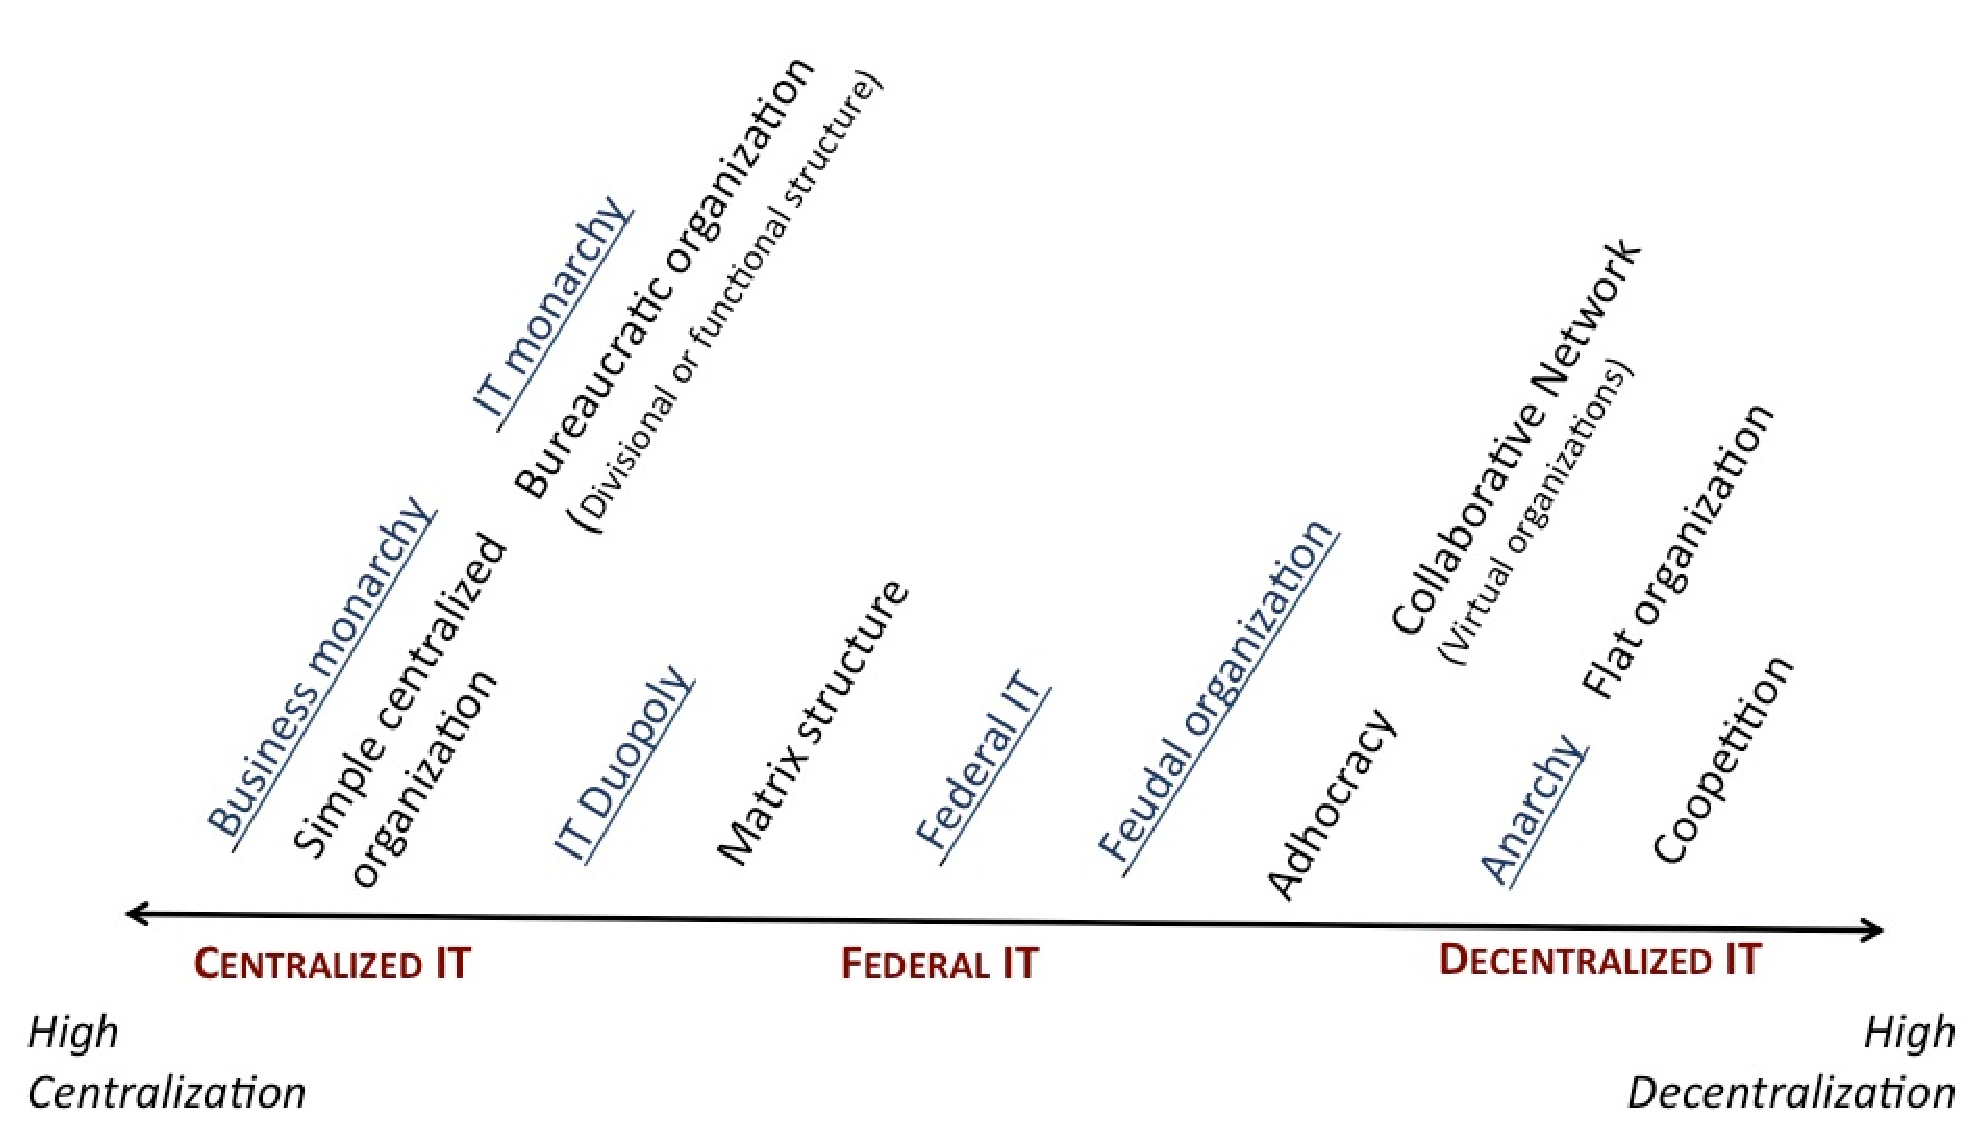
\includegraphics[scale=0.3]{taxonomy}
\caption{Organizational taxonomy: A Continuum From Centralized to Decentralized}
\label{fig:taxonomy}
\end{figure}

%TODO reflect in method

\paragraph*{Role of EA}

As detailed in Section \ref{sec:ea}, Enterprise Architecture is a discipline that allows an organization to construct and evolve its IT according to its needs. It provides a methodology and sets up a framework for assessing the current state of IT (architecture As-Is), for agreeing upon and communicating its future state (architecture To-Be), for planning, and for carrying out this transformation. By providing this framework, the modern EA frameworks of TOGAF, Zachman and FEA aim to solve the problem of business-IT alignment from the ground up through proper design. 

\paragraph*{The Problem} 

The EA frameworks of TOGAF, Zachman and FEA are primarily supportive of organizations with an structural form on the High Centralization end of the centralization continuum (Figure \ref{fig:taxonomy}). This is a problem for organizations on the High Decentralization end of the spectrum, who will likely encounter issues if they implement EA as it is currently described in TOGAF, Zachman, and FEA. Therefore, the addition of specific guidelines to these frameworks that are supportive of decentralization would improve their support of decentralized organizations. 


% **********************************************************************
% **********************************************************************
% **********************************************************************

\subsubsection{Motivate problem} %WHY PROBLEM IN IMPORTANT/RELEVANT
%TODO reflect in method

The problem of EA frameworks not being ideally suited for organizations on the High Decentralization end of the spectrum is important because: 1) organizations are becoming increasingly decentralized~\cite{acemoglu2007technology,fulk1995}, and 2) like centralized organizations, decentralized organizations can potentially benefit from the practice of EA.

Organizations on the High Centralization end of the continuum fail to adapt to dynamic environments due to their inertia in decision making and lack of agility \cite{fulk1995,pearlson2009}. As a result, organizations are moving towards High Decentralization, with organizational structures such as Collaborative Networks \cite{Camarinha-Matos2005} and Flat, where organizational subunits and individuals are being given an increasing amount of autonomy and control. Decentralized structures support transparent or dynamically changing boundaries, agile processes, interactions aligned in real-time with changing business conditions, virtual collaborations; all of which are technology-enabled capabilities~\cite{applegate1988,fulk1995}.


Decentralization means a significant change from the traditional management and operation styles of an organization and requires major changes in organizational processes. It transforms the role of authority and makes relationships inside and between different subunits much more complex. Planning and governance in different functional areas, including IT, is no longer centrally ensured. As a consequence, collaboration and information sharing between subunits gain extreme importance. This is evident in the challenges of decentralized organizations outlined in~\cite{caruso2008boundaries}.  

%TODO add more sources re: importance of communication/information sharing

While technology serves as an important catalyst for organizational transformations, it is important to utilize the right IT resources in a manner that is supportive of the organization. To accomplish this in decentralized organizations, novel EA processes, principles and concepts are needed to both handle the IT resources and to foster business/ICT co-evolution in decentralized environments. The de-facto EA frameworks rely on organizational properties that are becoming obsolete with progressive decentralization.  Due to this, implementation of these frameworks in decentralized organization becomes difficult and inefficient and the role of EA as a driver for IT transformations is becoming compromised. In order to deal with progressive decentralization, some changes or additions to these EA frameworks are necessary in order to improve their support for decentralization.



% **********************************************************************
% **********************************************************************
% **********************************************************************

\subsubsection{Find root causes}


The root cause of the discrepancy between current EA frameworks and decentralization lies in the fact that centralized and decentralized organizations have significantly different properties that are not always fully supported by EA. This section outlines these properties and specific areas of TOGAF, Zachman, and FEA that are supportive and not supportive of them. 

\paragraph*{Properties that differ between centralized and decentralized organizations}

A number of key properties of organizations and how they can differ between centralized and decentralized organizations have been identified.  These properties are detailed in Table \ref{org_characteristics}.

\begin{table}
\caption{Organizational Properties}
\label{org_characteristics}
%%\begin{tabular}{l p{0.28\textwidth}}
\begin{tabular}{ | p{0.25\textwidth} | p{0.35\textwidth}| p{0.35\textwidth} |}
%
\hline
%
\textbf{Property} & 
\textbf{Centralized} &
\textbf{Decentralized}  \\
%
\hline
%
Geographical dispersion \cite{luthans2006} & 
Single location &
Geographically distributed with a reliance on IS to work together \cite{applegate1988} \\
%
\hline
%
Coordination: authority, decision rights, standards and regulations & 
\textit{Vertical coordination}: decision rights are strictly defined and work their way down from the top \cite{Weill2004,pearlson2009}; strict governance and control by upper management \cite{pearlson2009,applegate1988}; rigid structuring of accountability, roles and responsibilities \cite{applegate1988}; standard methods and procedures \cite{mintzberg1981}; homogeneous goals set by high-level authorities \cite{Bolman2008} &
\textit{Lateral coordination}: authority and decision-making rights are pushed down to the level of groups, units or even individuals \cite{Weill2004,pearlson2009,robbins1997,Camarinha-Matos2005}; individuals can define their own roles and responsibilities \cite{valveHandbook}; heterogeneous goals, but individual entities in the organization are collaboratively working towards some common or complementing ones~\cite{Camarinha-Matos2005} \\
%
\hline
%
Communication patterns  & 
Communication patterns follow the hierarchy \cite{pearlson2009,applegate1988}; direct interactions and communications are often unnecessary \cite{thompson1967}; &
Informal communication lines~\cite{pearlson2009}; flexible, constantly changing communication lines~\cite{ahuja1998network}; fluid, project oriented teams.~\cite{applegate1988} \\
%
\hline
%
\end{tabular}
\end{table}



\paragraph*{TOGAF: Concepts supporting centralized organizations}

\subparagraph*{EA Method and EA Engine}
TOGAF outlines a formal approach to architecture governance which involves the setting up of an Architecture Board ``to oversee the implementation of the [architecture] strategy''~\cite[Ch. 47]{togaf9.1}. This board has an important role in Architecture Governance, such as ``[p]roviding the basis for all decision-making with regard to the architectures''~\cite[Ch. 47]{togaf9.1} and enforcing architecture compliance. 

Architecture board concept suits well for the organization with strong centralization in IT (Centralized IT to Federal IT in Fig. \ref{fig:taxonomy}.  Having a single entity responsible for high-level decision making is an aspect of vertical coordination  and as such,  fits in with the concept of a Centralized IT organization. TOGAF does suggest that the board has enterprise-wide representation~\cite[Ch. 47]{togaf9.1} which may support some level of decentralization, however it suggests the representation comes in the form of ``senior managers''; a concept which is again characteristic of vertical coordination. 

Throughout TOGAF, references are made to the existence of a bureaucratic or hierarchical centralized structure in place: 

For example, an important part of the preliminary phase is to set up a \textit{formal governance framework} for all architectural material, a concept that is related to the rigid forms of traditional organizational structure. 

Another example: after the completion of ``Phase A: Architecture Vision'', TOGAF requires approval of the current vision of the architecture. This requirement of approval assumes the existence of someone with a higher level of decision-making authority to give approval. 

A third example is an entire set of architectures at the strategic level of the Architecture Landscape which is meant for the ``executive level''~\cite[Ch. 20]{togaf9.1}.

\subparagraph*{EA Description}
TOGAF suggests the development of architecture principles that ``...define the underlying general rules and guidelines for the use and deployment of all IT resources and assets across the enterprise''~\cite[Ch. 23]{togaf9.1}. Having a set of principles that is applied to an entire organization is characteristic of vertical coordination and therefore supportive of centralization. 

TOGAF includes the concept of an Architecture Repository, which is to hold the entirety of the Architecture Landscape in addition to other architecture-related information. The idea of a single place to store all information is highly supportive of centralization. 

\paragraph*{TOGAF: Concepts supporting decentralized organizations}
\subparagraph*{EA Method and EA Engine}
TOGAF primarily supports some level of lateral coordination and decentralization through the concept of \textit{partitions}. It suggests dividing the Architecture Landscape into separate parts in order to support multiple architecture teams working concurrently and conflicting architectures in different organizational units. This enables ``federated architectures — independently developed, maintained, and managed architectures that are subsequently integrated within an integration framework''~\cite[Ch. 40.3]{togaf9.1}. 

Furthermore, ``[f]ederated architectures typically are used in governments and conglomerates, where the separate organizational units need separate architectures''~\cite[Ch. 40.3]{togaf9.1}. This supports the idea of different organizational units developing their own individual architectures. The mechanism for integrating the individual architectures under the roof of the corporate architecture is not explicit. 

TOGAF additionally indirectly supports decentralization through the suggestion that the entire TOGAF process be\textit{ tailored to fit the needs of the enterprise}. This is done in the preliminary phase of the ADM. This allows TOGAF to support any kind of enterprise, however, the guidelines provided for this are minimal. 

\paragraph*{Zachman: Concepts supporting centralized organizations}
%Limited perspectives?
\subparagraph*{EA Description}
The Zachman Framework aims to model a complete enterprise in a single, ``periodic table of elements''~\cite{Bente2012}. It attempts to break down an enterprise into a matrix of 36 elements, with alignment and composite integration relations defined between these elements. 

The perspectives of Zachman Framework line up with a bureaucratic organizational structure: the defined views (from executive to user) constitute an explicit organizational hierarchy. Clear separation between domains make this framework suitable for matrix organizations as well. 
%(e.g. executive and business management perspectives).

The lack of flexibility in definition of domains and views and the requirement to fill in the matrix - is perhaps the Zachman Frameworks main shortcoming with respect to decentralization. A primary aspect of decentralized organizations is their high level of flexibility. For a decentralized organization where both roles and domains are not uniformly defined (implicit) for subunits, the use of the Zachman Framework becomes difficult if at all possible.

\subparagraph*{EA Method and EA Engine}

Providing a schema for organizing architectural artifacts of an enterprise, the Zachman Framework does not imply any particular method for collecting these artifacts (what we call EA Method in Fig. \ref{fig:EA_general} ).
Neither is suggests the set of structures that we call EA Engine. 

Therefore, tailoring and  implementation of Zachman framework for a concrete organizational structure depends on experience of the EA (consultancy) team.

To summarize, the Zachman Framework provides a detailed taxonomy of EA artifacts that supports a hierarchical view on the organization. The application of this framework in decentralized (flat, adhocracy) organizations remains unclear.

\paragraph*{FEA: Concepts supporting centralized organizations}
\subparagraph*{EA Description}
Through the use of a common set of \textit{reference models}, FEA prescribes standards that are to be followed throughout the organization. This vertical coordination limits the flexibility that the individual organizational units have and makes this framework suitable for bureaucratic organizations with a high level of standardization in its processes.

In FEA, however, individual organizational units have the freedom to develop their own architecture as long as it fits in to the set standards. This lateral coordination supports some level of decentralization and is suitable for organizations with federal structure, where individual units have input into decisions. 

\subparagraph*{EA Method and EA Engine}

Segment architecture development is defined by FEA as a collaborative approach conducted by an integrated project team (IPT) comprising business subject matter experts, enterprise architects and technical subject matter experts.  FEA defines a set of segment architecture stakeholders and their roles (Table 2-2 in the document \cite{FEA_PMO2007}) whose ``commitment must be attained to support each step in this [development] process.''~\cite{FEA_PMO2007}.   For example, the role of senior management is defined to set the agency strategic goals; chief architect and EA team are appointed to supervise the architecture development process, coordinate the activities of other stakeholders and communicate and share the information between segments when needed; IPT activities and meetings are coordinated and managed by a Program Manager. The Program Manager should monitor progress, evaluate segment architecture completion and demonstrate results. These roles naturally line up with the centralized to federal organization of IT (Fig.\ref{fig:taxonomy}).
 
The mechanisms for enforcing standards and compliance, cross agency collaboration, and integrating the segment architectures under the roof of the corporate architecture is  assured by specific governance and management processes which, while implying different stakeholders, are based on vertical coordination. 

%FEA describes ``EA governance and management processes''~\cite[Sec. 2]{FEA_PMO2007} to control architecture development. These process are implemented to manage standards, enforce compliance, manage collaboration between agencies, approve architectures for implementation, and  manage business and IS requirements for managing EA change.

All steps of segment architecture development (Fig. \ref{fig:FEA_segmentDev}) involve/supervised by the Program manager and/or chief architect or Capital Planning and Investment Control (CPIC) lead, pointing on centralized management and budgeting.

Transition strategy is defined for the agency level though it is assessed on the global level. Governance-wide collaboration and reuse based on standards is outlined by FEA as an important part of RA transition strategy.

\paragraph*{FEA: Concepts supporting decentralized organizations}
\subparagraph*{EA Description}

The resulting segment architecture is positioned by FEA as a shared vision for business and IT transformation within a core mission area or common service. Each segment can have its own architecture that responds to its business needs.

\subparagraph*{EA Method and EA Engine}

The development of \textit{segment architectures} is described as a collaborative process between EA architects and other stakeholders. The accent is placed on the ``reconciliation'' of the segment architecture with an agency architecture and cross-agency initiative, emphasizing the importance of  cross-agency collaboration, common opportunities and initiatives.

Architectural analysis and architectural definition steps of segment architecture development (Fig. \ref{fig:FEA_segmentDev}) involve business owners at the agency level who define business and information management requirements for the segment. This allows to ensure the local, agency-level interests within a corporation. 

FEA is targeting the groups of independent federal agencies with an objective to increase their interoperability and quality of service they are offering for citizens. Among three EA frameworks considered in our study, FEA is the only one recognizing the need of inter- and intra-agency cooperation and communication. Nevertheless, many of the concepts on which the EA method and EA engine of FEA are grounded remain strongly centralized. Again, this supports our initial claim.

\begin{table}
\caption{Existing and Prospective support of Progressive Decentralization by EA frameworks}
\label{table:summary}
%%\begin{tabular}{l p{0.28\textwidth}}
\begin{tabular}{ | l | p{0.25\textwidth}| p{0.25\textwidth} | p{0.25\textwidth}|}
%
\hline
%
EA component: & 
\textbf{Existing support for centralized organizations} &
\textbf{Existing support for decentralized organizations} &  
\textbf{Applicable P2P principles for a solution} \\
%
\hline
%
\textbf{EA Method:} & 
Approval process based on hierarchy; architecture development is coordinated, supervised and evaluated by well-defined roles in a company (e.g. senior managers define strategic goals); EA teams coordinate architectural work and communicate results; results are controlled and evaluated centrally - by program manager) &
Federated architectures; possibility to adapt ADM for a specific organization; architecture development process involves multiple stakeholders & 
peer production principles for creation and evaluation of EA artifacts; P2P trust management replacing approval mechanism\\
%flexible ADM & peer production; P2P trust management\\
%
\hline
%
\textbf{EA Description:} & 
Strategic level architectures; hierarchy of architecture principles; a common set of reference models; hierarchical organization of EA artifacts with explicitly defined roles and domains (Zachman) &
Architecture partitions; architecture reference models; segment architecture; the concept of ``shared vision'' & 
User-driven content submission and change management of the content (i.e. the structure is defined by the users)\\
%
\hline
%
%
\textbf{EA Engine:} &
Architecture board; vertically coordinated governance framework; common set of principles for entire organization (i.e global commitment is taken for granted); centrally managed architecture repository &
integration of various (segment) architectures is assured by (centralized) management and governance &
Peer production for relevance/accreditation (e.g. decision making in budgeting, strategy, opportunity evaluation, solution evaluation); user-driven content submission and change management of the content; P2P trust management\\
%
\hline
%
\end{tabular}
\end{table}


% **********************************************************************
% **********************************************************************
% **********************************************************************


\subsection{Iteration 2}

\subsubsection*{Define Precisely}

DSV has decent/federated structure, needs supporting EA

% **********************************************************************
% **********************************************************************
% **********************************************************************

\subsubsection*{Motivate problem}

% **********************************************************************
% **********************************************************************
% **********************************************************************

\subsubsection*{Find root causes}




%
%
%
% RANDOM NOTES
%
%

%%%% applegate
%%%% In fact, the need to be responsive led to even more decentralized decision making.
%%%%Today there is
%%%%a third option: technology-driven control systems ,
%%%%that support the flexibility and responsiveness of a
%%%%decentralized organization as well as the integration
%%%%and control of a centralized organization.
%%%
%%%%At the same time, the business environment is
%%%%changing ever faster, and organizations must be more
%%%%responsive to it. Yet certain facts of life restrain them
%%%%from doing so. Companies want to be more flexible,
%%%%yet job descriptions, compensation schemes, and
%%%%control mechanisms are rigid. They want to use their
%%%%resources effectively, yet it's not always clear who
%%%%can contribute most to a project, especially among
%%%%people in different functional areas. They want to be
%%%%productive, but every time an employee goes to another
%%%%company, a little bit of corporate history and
%%%%experience walks out the door.
%%%%
%%%%With the help of technology; managers will be able
%%%%to overcome these problems and make their organizations
%%%%far more responsive than they are today. We
%%%%can look forward, in fact, to an era in which managers
%%%%will do the shaping. Large organization or small, centralized
%%%%or not- business leaders will have options
%%%%they've never had before. The technology will be
%%%%there to tum the vision into reality and to change it as
%%%%circumstances evolve. With that in mind, making a
%%%%next round of predictions and waiting to see if they
%%%%come true seems too passive. It makes more sense to
%%%%begin thinking about the kind of organization we
%%%%want and taking the steps necessary to prepare for it
%%%
%%%%In the cluster organization, groups of people will
%%%%work together to solve business problems or define a
%%%%process and will then disband when the job is done.
%%%%Team members may be geographically dispersed and
%%%%unacquainted with each other, but information and
%%%%communication systems will enable those with
%%%%complementary skills to work together.
%%%
%%%%In the network organization,
%%%%rigid hierarchies are replaced by formal !
%%%%and informal communication networks that connect
%%%%all parts of the company. In the adhocracy, a set of
%%%%project-oriented work groups replace the hierarchy.
%%%%Both of these forms are well known for their flexibility
%%%%and adaptiveness. The Manned Space Flight Center
%%%%of NASA, an example of an adhocracy, changed its
%%%%organization structure 17 times in the first 8 years of
%%%%its existence.
%%%%
%%%%In what will be an even faster changing world than
%%%%the one we now know, businesses of all sizes will
%%%%need the ability to adapt to the dynamics of the external
%%%%environment. Automated information and communication
%%%%networks will support the sharing of
%%%%information throughout a large, widely dispersed,
%%%%complex company. The systems will form the organization's
%%%%infrastructure and change the role of formal
%%%%reporting procedures.
%%%%
%%%%Even in large corporations,
%%%%each individual will be able to communicate with
%%%%any other-just as if he or she worked in a small
%%%%company